\chapter{Le trasformazioni di Lorentz }
In relatività le trasformazioni di Galileo sono sostituite dalle trasformazioni di Lorentz, prima di vederle nel dettaglio bisogna ricordarsi 
che le grandezze che ci interessano non sono più i semplici vettori ma i \textbf{ quadrivettori contravarianti } che definiamo nel seguente modo :
\begin{center}
        
        $ \vectorbold{X^{\mu}} = \begin{pmatrix} ct\\ \va{x} \end{pmatrix} $

\end{center}
Tale notazione evidenzia come i quadrivettori siano divisi in una parte temporale ( la prima componente ) e componenti spaziali ( vettore tridimensionale ), 
tali quaterne di valori trasformano, nel passaggio da un sistema di riferimento ad un altro, tramite le trasformazioni di Lorentz. \\
La metrica dei quadrivettori non è la metrica Euclidea bensì quella di \textbf{Minkowski}, se definiamo infatti due quadrivettori 
\begin{align*}
        \vectorbold{A^{\mu}} = \begin{pmatrix} a_0\\a_1\\a_2\\a_3\end{pmatrix}
        \
        \vectorbold{B^{\mu}} = \begin{pmatrix} b_0\\b_1\\b_2\\b_3\end{pmatrix}
\end{align*}
Allora il prodotto fra i due si definisce come :
\begin{align*}
        \vectorbold{A^{\mu}}\vdot\vectorbold{B_{\mu}} = a_0b_0 - a_1b_1 - a_2b_2 - a_3b_3
\end{align*}
dove $\vectorbold{B_{\mu}}$ non è altro che il \textbf{quadrivettore covariante} ossia il quadrivettore contravariante ma con il segno della parte spaziale opposto .\\
D'ora in avanti indicheremo $\vectorbold{X} \equiv \vb{X^{\mu}} $.
\newpage

\section{Trasformazione delle coordinate}
Supponiamo di avere un sistema di riferimento $\mathbb O$ fermo ( sistema del laboratorio ) e un sistema $\mathbb O^{'} $ in movimento 
con velocità V come in figura.\\

\begin{figure}[!h]
        \centering 
        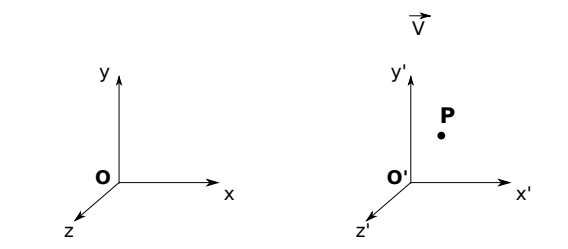
\includegraphics[scale=0.8]{SistemaRiferimento}
        \caption{Sistemi di riferimento}
\end{figure}
Indichiamo con $\vb{X}$ il quadrivettore posizione del punto \textbf{P} rispetto a $\mathbb O$ e $\vb{X^\prime}$ rispetto a $\mathbb O^\prime$, le coordinate di 
$\vb{X^\prime}$ si trovano rispetto alle coordinate misurate in $\mathbb O^\prime$ nel seguente modo : 
\begin{align*}
        \vectorbold{X^\prime} = \vb{\Lambda^{\mu}_{\nu}} \vb{X} 
\end{align*} 
dove $\vb{\Lambda^{\mu}_{\nu}}$ rappresenta la matrice della trasformazione di Lorentz lungo asse x data da : 
\begin{align*}
        \vb{\Lambda^{\mu}_{\nu}} = \begin{pmatrix} \gamma & -\gamma\beta & 0 & 0 \\ -\gamma\beta & \gamma & 0 & 0 \\ 0 & 0 & 1 & 0 \\ 0 & 0 & 0 & 1 \end{pmatrix} \tag*{$\beta = \frac{V}{c}$ \ $\gamma = \frac{1}{\sqrt{1-\beta^2}}$}
\end{align*}
si ottiene quindi il seguente sistema : 
\begin{equation*}
\left\{ \begin{aligned}
        ct^{\prime}&=\gamma(ct - \beta x) \\
        x^{\prime}&= \gamma( x - ct\beta ) \\
        y^{\prime}&= y \\
        z^{\prime} &= z
  \end{aligned}
  \right.
\end{equation*}
\begin{tcolorbox}[colback=red!5!white,colframe=red!50!black,title=ATTENZIONE !]
Se il cambio di sistema di riferimento si fa dal sistema in moto al sistema di riferimento del laboratorio allora $\beta$ cambia di segno 
\end{tcolorbox}
\newpage
\section{Trasformazione delle velocità}
Per capire bene le trasformazioni delle velocità conviene vedere un esercizio.\\
\begin{center}\textbf{Esercizio  }\end{center} 
Un uomo in automobile viaggia ad una velocità di $\frac{3}{4}c$, viene inseguito da un'altra automobile che va alla velocità di $\frac{1}{2}c$ 
la quale spara un proiettile che va alla velocità di $\frac{1}{3}c$.
Il proiettile raggiunge l'auto ? \\
\begin{center}\textbf{Soluzione}\end{center}
La questione è tutta basata sulle trasformazioni delle velocità in relatività, le troveremo tramite le trasformazioni di Lorentz viste prima, 
un commento prima di trovarle : 
\\
\begin{tcolorbox}[colback=red!5!white,colframe=red!50!black,title=ATTENZIONE !]
Bisogna capire bene i sistemi di riferimento, nel nostro caso stiamo osservando le macchine che corrono, noi siamo il laboratorio ( sistema fermo )
il problema è che la velocità del proiettile è calcolata nel sistema di riferimento in moto ( ossia la macchina che spara ), il gioco è tutto quì : 
trasformare la velocità del proiettile dal sistema di riferimento in moto a quello del laboratorio . 
\end{tcolorbox}
Partiamo dalla trasformazione di Lorentz per la posizione, come al solito identifichiamo con $x^{\prime}$ le coordinate del sistema di riferimento in moto : 
\begin{equation*}
\left\{ \begin{aligned}
                ct&=\gamma(ct^{\prime} + \beta x^{\prime}) \\
        x&= \gamma( x^{\prime} + ct\beta ) \\
        y&= y^{\prime} \\
        z&= z^{\prime}
  \end{aligned}
  \right.
\end{equation*}
Notare come c'è il cambio di segno dovuto al fatto che passiamo da sistema in moto a quello del laboratorio. \\
Passiamo ora agli infinitesimi : 
\begin{equation*}
        \left\{ \begin{aligned}
                        c\dd{t} &= \gamma c\dd{t^{\prime}} + \beta\gamma\dd{x^{\prime}} \\
                        \dd{x} &= \gamma\dd{x^{\prime}} + c\gamma\beta\dd{t^{\prime}} \\
                        \dd{y} &= \dd{y^{\prime}} \\
                        \dd{z} &= \dd{z^{\prime}} \\
                \end{aligned}
                \right.
\end{equation*}
Dividiamo ora ciascuna componente per $\dd{t}$ la cui espressione l'abbiamo ricavata sopra, dividiamo poi numeratore e denominatore per $\dd{t^{\prime}}$, sostiuiamo $ \frac{\dd{x^{\prime}}}{\dd{t^{\prime}}} \equiv \dd{v^{\prime}_{x}} $ eccetera, inoltre $\beta \equiv \frac{V}{c}$ 
dove V è la velocità del proiettile nel sistema in moto, si ottiene : 
\newpage
\begin{equation*}
        \left\{ \begin{aligned}
                        \frac{\dd{x}}{\dd{t}} &\equiv v_{x}&= \frac{\gamma v^{\prime}_{x} + \gamma V}{\gamma(c + \frac{V}{c}v^{\prime}_{x})} \\
                        \frac{\dd{y}}{\dd{t}} &\equiv v_{y}&= \frac{v^{\prime}_{y}}{\gamma(c + \frac{V}{c}v^{\prime}_{x})} \\
                        \frac{\dd{z}}{\dd{t}} &\equiv v_{z}&= \frac{v^{\prime}}{\gamma(c + \frac{V}{c}v^{\prime}_{x})}
            \end{aligned}
            \right.
\end{equation*}
Abbiamo così ottenuto le trasformazioni delle velocità : 
\begin{tcolorbox}[colback=red!5!white,colframe=red!50!black,title=ATTENZIONE !]
        \begin{equation*}
                \left\{ \begin{aligned}
                                v_{x} &= \frac{V + v^{\prime}_{x}}{c + \frac{V}{c^{2}}v^{\prime}_{x}/}\\
                                v_{y} &= \frac{v^{\prime}_{y}}{\gamma(c + \frac{V}{c}v^{\prime}_{x})} \\
                                v_{z}&= \frac{v^{\prime}}{\gamma(c + \frac{V}{c}v^{\prime}_{x})}
                        \end{aligned}
                        \right.
        \end{equation*}
        Ricorda sempre che stiamo passando dal moto al fermo !!!!!
\end{tcolorbox}
\newpage
